

Ziel dieses Projekts ist es asymptotisch exponentiell abfallende Funktionen auf dem unbeschränkten Intervall $[0, +\infty)$ numerisch zu integrieren. Dazu untersuchen wir zwei mögliche Strategien:

\begin{itemize}
    \item[(a)] Abschneiden des unbeschränkten Intervalls und Anwendung einer Quadraturformel für ein beschränktes Intervall $[0, T]$ für $T > 0$

    \item[(b)] Anwendung einer Gauß-Quadratur für die Gewichtsfunktion $w(x) = \exp(-x)$
\end{itemize}


\label{listing:1}


\subsection*{a)}
Sei $f: [0,+\infty) \rightarrow \mathbb{R}$ eine beschränkte Funktion, deren erste und zweite Ableitung ebenso beschränkt sind. Desweiteren definieren wir für eine Menge $M \subset [0,+\infty)$ das gewichtete Integral von $f$ mit
\[Q_M(f) := \int_M f(x)\exp(-x) dx.\]

Wir approximieren das Integral $Q_{[0,\infty)}(f)$ indem wir für ein $T > 0$ das Integral auf dem beschränkten Intervall $Q_{[0,T]}$ durch die summierte Trapezregel approximieren. 
Wir definieren $Q_{T,h}(f) := \frac{h}{2}\left(\exp(-0)f(0) + 2\sum_{j=1}^{N-1}\exp(-jh)f(jh)+\exp(-T)f(T)\right)$ und wollen nun eine Abschätzung des Fehlers herleiten.\\
Mit der Dreiecksungleichung erhalten wir:
\begin{equation*}
    |Q_{[0,\infty)}(f) - Q_{T,h}(f)| \leq |Q_{[0,\infty)}(f) - Q_{[0,T)}(f)| + |Q_{[0,T)}(f) - Q_{T,h}(f)|
\end{equation*}
Der erste Term lässt sich direkt berechnen:
\begin{equation*}
    |Q_{[0,\infty)}(f) - Q_{[0,T)}(f)| = \int_{T}^{\infty}\exp(-x)f(x)dx = \exp(-T)
\end{equation*}
Dank Satz 4.8. aus dem Vorlesungsskript wissen wir:
\begin{equation*}
    |Q_{[0,T)}(f) - Q_{T,h}(f)| \leq \frac{T}{12}h^2 \sup_{x\in[0,T]}\{\exp(-x)( f^{''}(x)-2f^{'}(x)+f(x))\}
\end{equation*}
Also erhalten wir mit $C_2 := \frac{\sup_{x\in[0,T]}\{\exp(-x)( f^{''}(x)-2f^{'}(x)+f(x))\}}{12}$:
\begin{equation*}
    |Q_{[0,\infty)}(f) - Q_{T,h}(f)| \leq \exp(-T) + C_2Th^2
\end{equation*}

\subsection*{b)}
Nun gilt es die theoretischen Resultate aus Aufgabe a) zu implementieren und durch geeignete numerische Beispiele zu testen.
Wir haben uns für die Programmiersprache Python entschieden. 
\begin{lstlisting}[language=Python]
def trapez (f,N,T):
    x = np.linspace(0,T,N)
    summe = sum([f(x[i])*np.exp(-x[i]) for i in range(1,N-1)])
    trapez = 2*summe
    trapez += f(x[0])+f(x[N-1])*np.exp(-x[N-1])
    trapez *= (T/(2*(N-1)))
    return trapez
\end{lstlisting}
Wir betrachten die Funktion $f: x \mapsto \sin(x)$ mit
\[\int_{0}^{\infty}\sin(x)\exp(-x)dx = \frac{1}{2}\]
In Abbildung 1 sieht man den Fehler in Abhängigkeit von h anhand einigen ausgewählten, festen Werten für T.
In Abbildung 2 ist der Fehler abhängig von T mit einigen festen Werten für h zu sehen.\\
Jetzt wollen wir das optimale h in Abhängigkeit von T finden, dass abhängig von der Anzahl der Funktionsauswertungen den geringsten Fehler liefert. In Abbildung 1 sieht man, dass bei festem T irgendwann ein Punkt erreicht ist, ab dem der Fehler abhängig von T dominiert und eine weitere Verkleinerung der Teil-Intervalllänge h keine merkbare Verbesserung des Fehlers herbeiführen würde.\\ Ebenso verhält es sich in Abbildung 2, wobei hier ab einem gewissen Punkt eine weitere Vergrößerung von T, sogar zu einer Verschlechterung des Fehlers führen würde. Daher scheint es am sinnvollsten, h so zu wählen, dass sich die Fehler $T\epsilon_h$ und $\epsilon_T$ die Waage erhalten. Lösen wir nun nach h auf, erhalten wir: $h = \frac{\exp(-T)}{T}$.\\
Damit erhalten wir folgende Konvergenzplots:
\begin{figure}
    \centering
    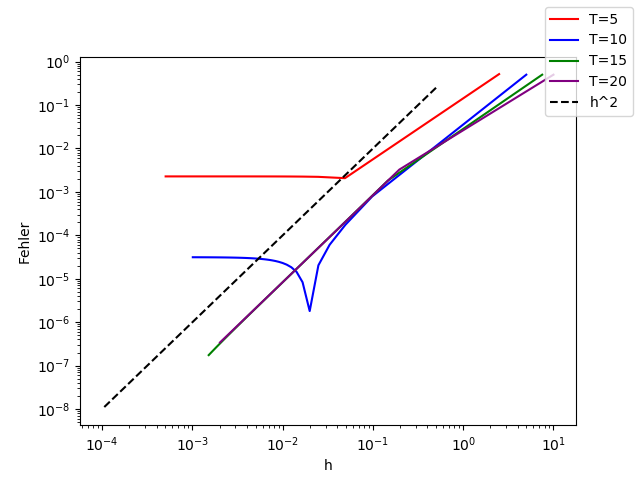
\includegraphics[width=1.2\linewidth]{fehler_h.png}
    \caption{T fest, h variabel}
    \label{fig:my_label}
\end{figure}



\begin{figure}[hbt!]
    \centering
    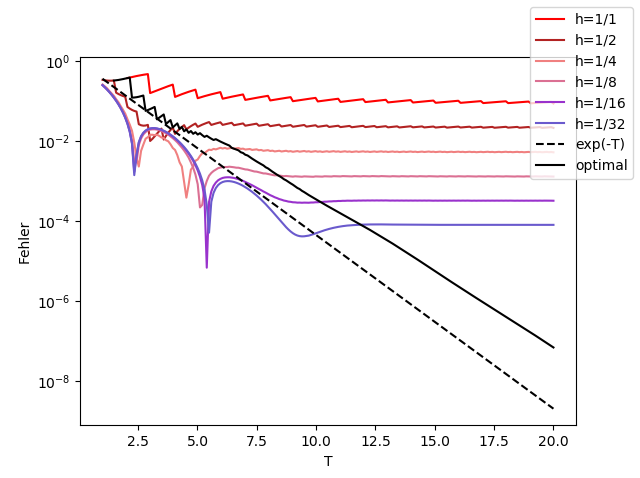
\includegraphics[width=1.2\linewidth]{fehler_T.png}
    \caption{h fest, T variabel}
    \label{fig:my_label}
\end{figure}



\begin{figure}
    \centering
    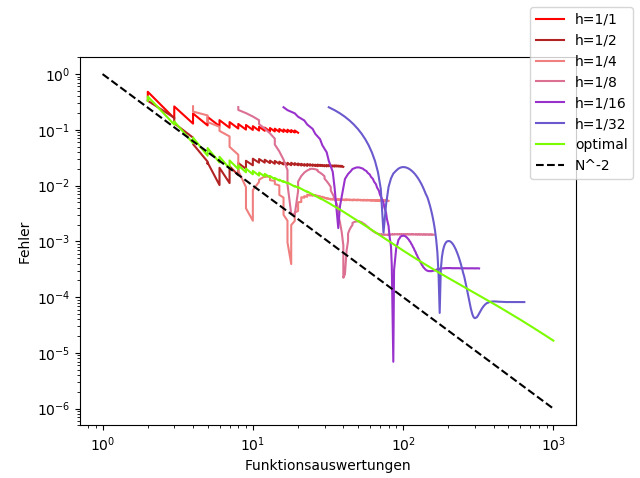
\includegraphics[width=1.2\linewidth]{optimal.png}
    \caption{Vergleich: feste h gegen optimales h }
    \label{fig:my_label}
\end{figure}
\pagebreak
\FloatBarrier
\subsection*{c)}
Um uns als nächstes der zweiten möglichen Strategie zuwenden zu können, müssen wir vorerst mit etwas theoretischer Vorarbeit starten, um die benötigten Quadraturpunkte und Quadraturgewichte für die Gaussquadratur berechnen zu können.
In Übungsaufgabe 39 wurde gezeigt, dass die Polynome $p_j$ gegeben durch die Dreitermrekursion
\[ p_0(x) = 1, p_1(x) = x - 1, p_{n+1}(x) = (x - 2n - 1)p_n(x) - n^2P_{n-1}(x)\]
die Orthogonalpolynome zur Gewichtsfunktion $\omega(x) = \exp(x)$ sind. Wir zeigen noch, dass die Nullstellen von $p_n$ genau die Eigenwerte der Matrix
\[T_n = \left(\begin{array}{rrrr}                                
1 & -1 & & \\                                               
-1 & 3 &\ddots& \\                                               
&\ddots&\ddots& -n + 1 \\
& & -n + 1 & 2n - 1 \\
\end{array}\right)\]
sind und dass die zugehörigen Gauß-Gewichte durch die Quadrate der ersten Einträgen der zugehörigen normierten Eigenvektoren sind.

\begin{align*}
\left(
\begin{array}{rrrr}                                
1 & -1 & & \\                                               
-1 & 3 &\ddots& \\                                               
&\ddots&\ddots& -n + 1 \\
& & -n + 1 & 2n - 1 \\
\end{array}
\right)
\cdot
\left(
\begin{array}{c}
    \tau_{0}p_{0}(x_{k})  \\
    \tau_{1}p_{1}(x_{k}) \\
    \vdots \\
    \tau_{n-1}p_{n-1}(x_{k})
\end{array}
\right) =
\end{align*}
\begin{align*}
\left(
\begin{array}{c}
    \tau_{0} - \tau_{1}p_{1}(x_{k}) \\
    \vdots \\
    -(i-1)\tau_{i-2}p_{i-2}(x_{x}) + (2i-1)\tau_{i-1}p_{i-1}(x_{k})+(-i)\tau_{i}p_{i}(x_{k}) \\
    \vdots \\
    -(n-1) \tau_{n-2}p_{n-2}(x_{x}) + (2n-1)\tau_{n-1}p_{n-1}(x_{k})
\end{array}
\right)
\end{align*}
Betrachten wir nun die i-te Zeile für $1 < i < n$ und gehen mit $p_{i}$ in die Rekursion \\
\begin{align*}
    &= \cdots + (-i)\tau_{i}[(x_{k}-2(i-1)-1)p_{i-1}(x_{k})-(i-1)^{2}p_{i-2}(x_{k})] \\
    &= \cdots + (-i)\tau_{i}[(x_{k}-(2i-1))p_{i-1}(x_{k})-(i-1)^{2}p_{i-2}(x_{k})]
\end{align*}
Durch Einsetzen erhalten wir $(-i)\tau_{i}=\tau_{i-1}$ und $\tau_{i-1}(i-1)^{2}= -(i-1)\tau_{i-2}$ und somit ergibt sich nur noch  $x_{k}\tau_{i-1}p_{i-1}(x_{k})$ in der i-ten Zeile. In der ersten Zeile erhält man durch Einsetzen wiederum $x_{k}\tau_{0}$. \\
Wir wissen, dass $x_{k}$ die Nullstellen von $p_{n}$ sind, somit können wir in der letzten Zeile die Terme $-n\tau_{n}p_{n}(x_{k})+n\tau_{n}p_{n}(x_{k})$ hinzufügen:
\begin{align*}
    -(n-1) \tau_{n-2}p_{n-2}(x_{x}) + (2n-1)\tau_{n-1}p_{n-1}(x_{k})-n\tau_{n}p_{n}(x_{k})+n\tau_{n}p_{n}(x_{k})
\end{align*}
Durch das Ergebnis von vorhin und mit dem Wissen, dass $p_{n}(x_{k})=0$, erhalten wir für die letzte Zeile $x_{k}\tau_{n-1}p_{n-1}(x_{k})$. Somit haben wir gezeigt, dass $x_{k}$ Eigenwerte von $T_{n}$ sind. \\ 
Im zweiten Teil zeigen wir, dass die Quadraturgewichte durch $w_{k,n} = \frac{1}{\lVert\nu_{k,n}\rVert^2}$ gegeben sind. $w_{k,n}$ sind die Gewichte der Gauss-Quadratur zur Gewichtsfunktion $e^{-x}$.
\begin{align*}
    \sum_{j=0}^{n-1}\sum_{l=0}^{n}w_{l,n}\tau_j^2p_j(x_k)p_j(x_l)= \sum_{j=0}^{n-1}\left(\sum_{l=0}^{n}w_{l,n}p_j(x_l)\right)\tau_j^2p_j(x_k) = \\
    \sum_{j=0}^{n-1}\left(\int_{0}^{\infty}e^{-x}p_{j}(x)dx\right)\tau_j^2p_j(x_k) = \sum_{j=0}^{n-1}\left(\int_{0}^{\infty}e^{-x}p_{j}(x)p_{0}(x)dx\right)\tau_j^2p_j(x_k)
\end{align*}
Wir wissen, dass $p_{j}(x)$ untereinander orthogonal zur Gewichtsfunktion $e^{-x}$ sind. Somit sind alle Summanden $=0$, ausser wenn $j=0$. Das Integral von $\int_{0}^{\infty}e^{-x}dx$ beträgt 1.
\begin{align*}
 \sum_{j=0}^{n-1}\left(\int_{0}^{\infty}e^{-x}p_{j}(x)p_{0}(x)dx\right)\tau_j^2p_j(x_k)=1\cdot\tau_{0}^{2}p_{0}(x_{k})=1   
\end{align*}

Gleichzeitig erhalten wir unter der Ausnutzung, dass die Eigenvektoren einer symmetrischen Matrix bezüglich der euklidischen Skalarprodukts orthogonal aufeinander stehen:
\begin{align*}
     \sum_{j=0}^{n-1}\sum_{l=0}^{n}w_{l,n}\tau_j^2p_j(x_k)p_j(x_l) = & \sum_{l=0}^{n}w_{l,n}\sum_{j=0}^{n-1}\tau_jp_j(x_k)\tau_jp_j(x_l) = \\
     \sum_{l=0}^{n}w_{l,n}\sum_{j=0}^{n-1}\nu_{k,n}^{\top}\nu_{l,n} = &
      ~w_{k,n}\nu_{k,n}^{\top}\nu_{k,n} = w_{k,n}\lVert\nu_{k,n}\rVert^2
\end{align*}
Damit erhalten wir: $w_{k,n} = \frac{1}{\lVert\nu_{k,n}\rVert^2}$

\subsection*{d)}
Nachdem wir Satz 4.23 hinsichtlich der Gewichtsfunktion $w(x)=\exp(-x)$ gezeigt haben, können wir somit die Gewichte ($\alpha_{j}$) der Gauß-Quadratur berechnen.
Mithilfe der Funktion numpy.linalg.eig lassen sich die Eigenwerte und die dazugehörigen normierten Eigenvektoren der Matrix $T_{n}$ berechnen. Da der erste Eintrag der normierten Eigenvektoren bereits $\frac{1}{\lVert\nu_{k,n}\rVert}$ beträgt, müssen wir ihn nur noch quadrieren um das gewünschte Gewicht zu erhalten.\\
Aus Satz 4.17 des Vorlesungsskripts wissen wir, dass die Quadraturpunkte durch die Nullstellen des orthogonalen Polynoms $p_n$ gegeben sind. Mit dem Ergebnis der vorigen Aufgabe wissen wir, dass die Nullstellen von $p_n$ genau die Eigenwerte der Matrix $T_n$ sind. Damit haben wir alles, was wir für die Implementierung der Gaussquadratur benötigen.\\
\begin{lstlisting}[language=Python]
def gauss(f,N):
    T = np.diag([2*i+1 for i in range(N)])
    T -= np.diag([i for i in range(1,N)],1)
    T -= np.diag([i for i in range(1,N)],-1)
    values, vectors = np.linalg.eig(T)
    alphas = [(vectors[0][i])**2 for i in range(N)]
    summe = sum([alphas[i]*f(values[i]) for i in range(N)])
    return summe, alphas, values
\end{lstlisting}
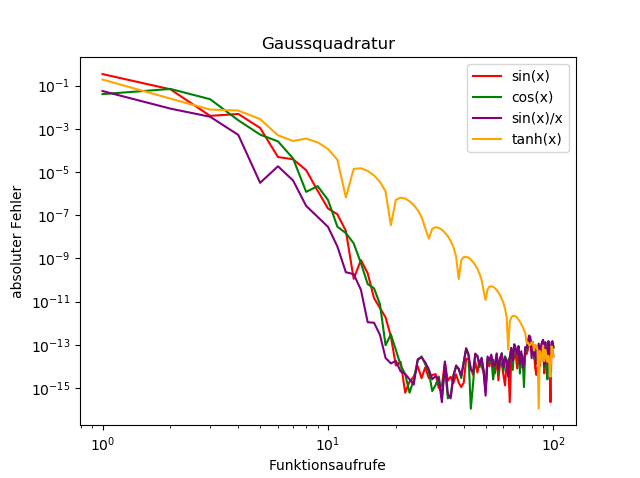
\includegraphics[width=1.2\linewidth]{gauss.png}
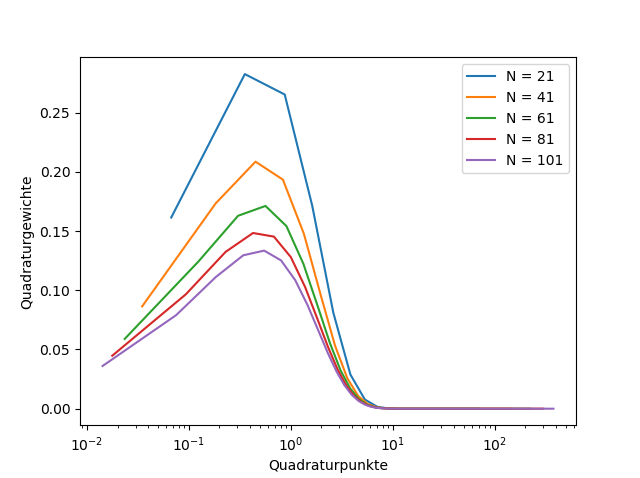
\includegraphics[width=1.2\linewidth]{punkte-gewichte.png}
Im ersten Plot sehen wir den Fehler der Quadratur anhand ausgewählter trigonometrischer Funktionen. In 3 von 4 Fällen sind wir bereits nach 20 Funktionsaufrufe im Bereich der Maschinengenauigkeit, was den Fehler betrifft, ledíglich beim Tangens Hyperbolicus schwächelt die Gaussquadratur ein wenig und bentötigt ungefähr 100 Funktionsaufrufe um mit dem Fehler in die Nähe der Maschinengenauigkeit zu kommen.\\
Im zweiten Plot werden die Stützstellen gegen ihre zugehörigen Gewichte geplottet. Man erkennt gut, dass Quadraturpunkte rund um 1 am höchsten gewichtet werden und für größere werdende Quadraturpunkte konvergieren die zugehörigen Gewichte schnell gegen Null. Wie man anschaulich erwarten würde, tragen Werte jenseits von 10 kaum mehr etwas zum Integral bei und werden dementsprechend verschwindend gering gewichtet. Auch interessant zu beobachten ist, dass die kleinste Nullstelle bei steigendem N immer näher an 0 herankommt.
\subsection*{e)}
Schlußendlich stellt sich die Frage, welcher der beiden Ansätze nun der effizientere sei. Dazu betrachten wir die Kovergenzplots beider Quadraturen anhand geeigneter Beispiele:
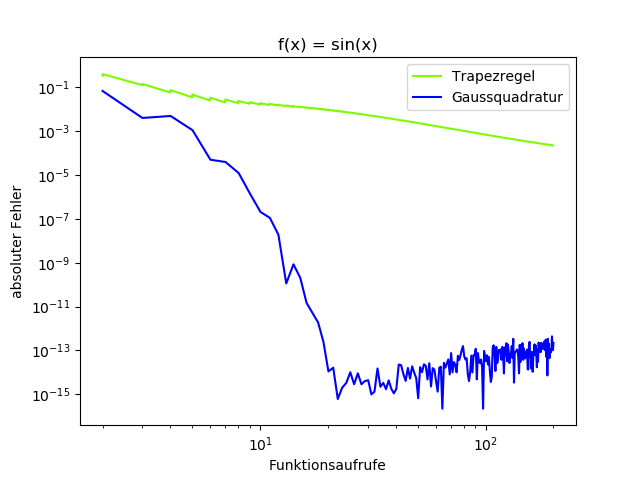
\includegraphics[width=0.5\linewidth]{gauss-trapez.png}
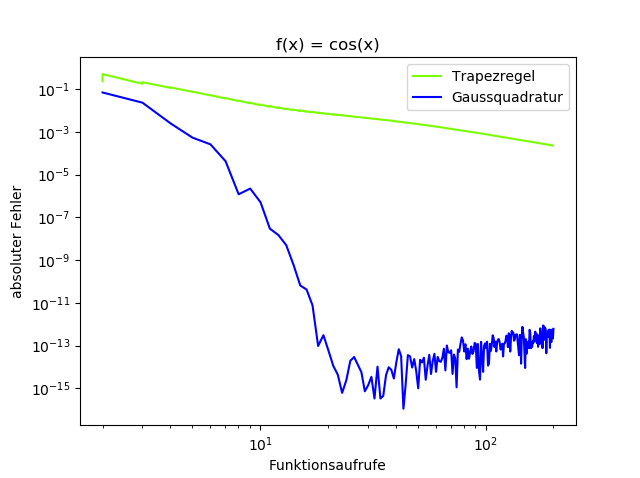
\includegraphics[width=0.5\linewidth]{gauss-trapez,cos.png}
Hier erkennt man, dass die Gauß-Quadratur ein deutlich schnelleres Konvergenzverhalten hat, als die summierte Trapezregel. Nach bereits ca. 20 Funktionsaufrufen sind wir im Bereich der Maschinengenauigkeit angelagt, ab dem natürlich keine weitere Verbesserung mehr möglich ist.

Wenn man nun als Gewichtsfunktion $\exp(-x^{2})$ wählt, liefert uns die Gaussquadratur bei den meisten Funktionen eine nur unwesentlich langsamere Konvergenz, allerdings mit Ausnahmen.
Bei der Sinus- und Cosinus-Funktion schneidet die Trapezregel wesentlich besser als erwartet ab und erreicht bereits nach ca. 20 Funktionsauswertungen einen Fehler in der Größenordnung der Maschinengenauigkeit. Beim Areasinh sehen wir allerdings wieder das zu erwartende Konvergenzverhalten der Trapezregel, klar geschlagen von der Gaussquadratur. Bei $f: x \mapsto \tanh(x^2)$ gewinnt allerdings wieder die Trapezregel. Noch interessanter wird die Geschichte bei $f: x \mapsto \text{arcosh}(x+1)$: Hier konvergieren beide Quadraturformeln mit der selben Geschwindigkeit, die Gaussquadratur ist lediglich um einen Faktor von ca. 100 besser. Bei der Funktion $f: x \mapsto \sin(\frac{1}{x})$ an der Stelle 0 gleich 0 gesetzt scheitern jedoch beide Formeln kläglich. Die letzten beiden Resultate lassen sich allerdings erklären, wenn man die Ableitung der Funktion in einer Umgebung von 0 betrachtet und feststellt, dass sie dort unbeschränkt ist.
\FloatBarrier
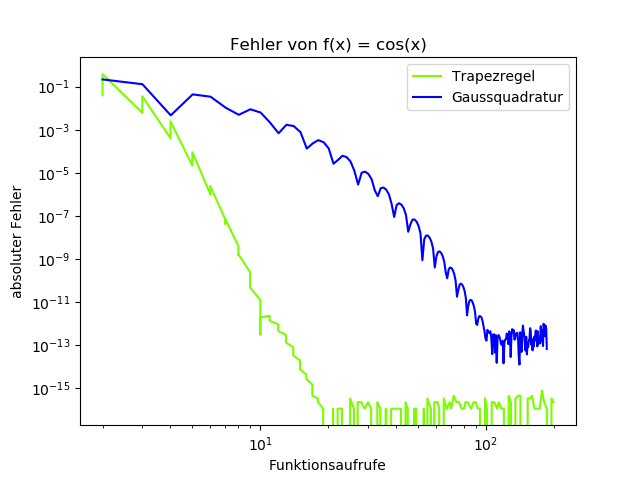
\includegraphics[width=0.5\linewidth]{gauss-trapez(-x^2),cos.png}
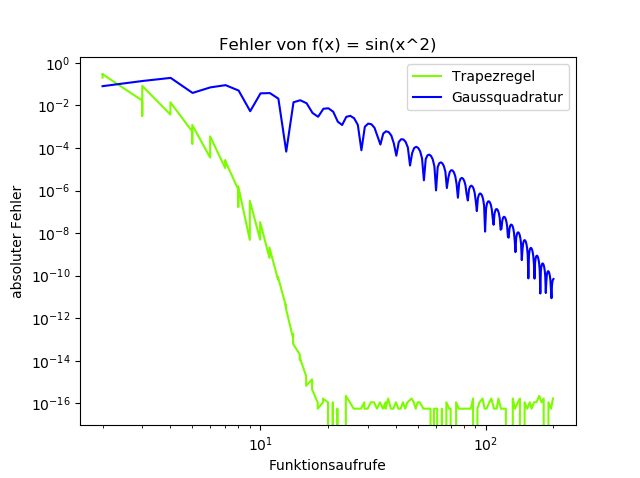
\includegraphics[width=0.5\linewidth]{gauss-trapez(-x^2),sin(x^2).png}
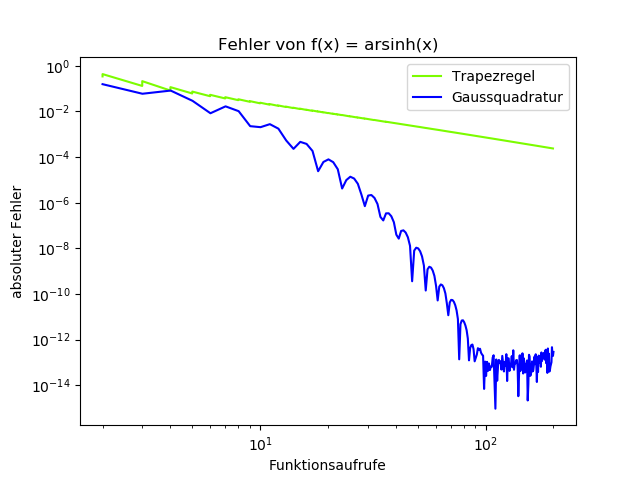
\includegraphics[width=0.5\linewidth]{gauss-trapez-arsinh.png}
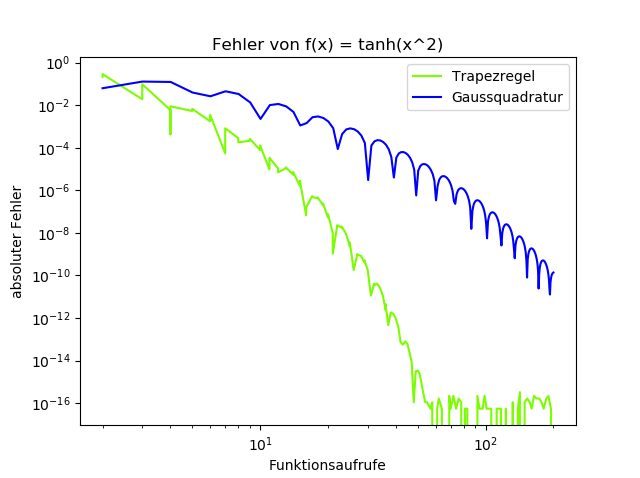
\includegraphics[width=0.5\linewidth]{gauss-trapez-tanh.png}
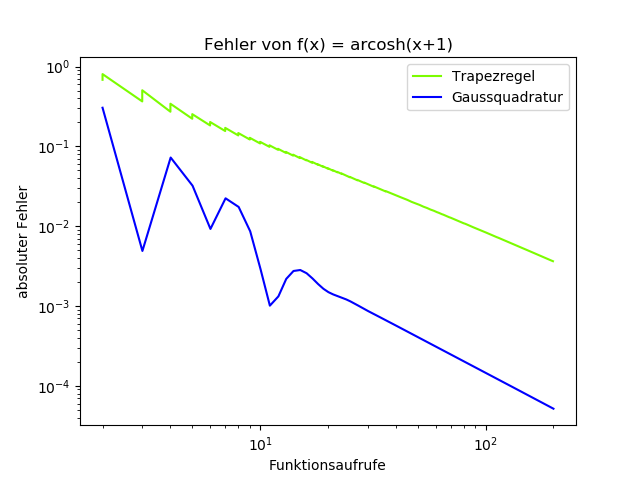
\includegraphics[width=0.5\linewidth]{gauss-trapez-arcosh.png}
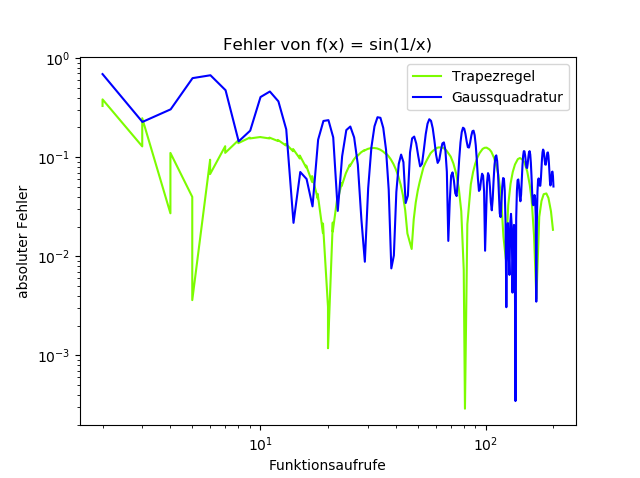
\includegraphics[width=0.5\linewidth]{gauss-trapez-sin.png}